\documentclass[a4paper]{report}
\usepackage[T1]{fontenc} 
\usepackage[utf8]{inputenc} 
\usepackage[backend=biber, style=numeric-comp]{biblatex}
\usepackage{csquotes}
\usepackage[portuguese]{babel} 
\usepackage{blindtext} 
\usepackage[printonlyused]{acronym}
\usepackage{hyperref} 
\usepackage{subfigure}
\usepackage{color,graphicx}
\usepackage{float}
\usepackage{url}
\usepackage{multicol}

\begin{document}

\def\titulo{DISPOSITIVOS DE ARMAZENAMENTO}
\def\data{19/11/2017}
\def\autores{João Tomás Simões, Martim Neves (Grupo 7)}
\def\autorescontactos{(88930) jtsimoes@ua.pt, (88904) martimfneves@ua.pt}
\def\versao{MIECT}
\def\departamento{Laboratórios de Informática (Turma 4)}
\def\empresa{Universidade de Aveiro}
\def\logotipo{ua.pdf}

\begin{titlepage}

\begin{center}

\vspace*{50mm}

{\Huge \titulo}\\ 

\vspace{10mm}

{\Large \empresa}\\

\vspace{10mm}

{\LARGE \autores}\\ 

\vspace{30mm}

\begin{figure}[h]
\center
\includegraphics{\logotipo}
\end{figure}

\vspace{30mm}
\end{center}

\begin{flushright}
\versao
\end{flushright}
\end{titlepage}


\title{
{\Huge\textbf{\titulo}}\\
\vspace{3mm}
{\Large \departamento\\ \empresa}
}

\author{
    \autores \\
    \autorescontactos
}

\date{\data}

\maketitle

\pagenumbering{roman}

\begin{abstract}

Nesta era digital, será que alguém já parou para pensar quantos bytes de informação o mundo armazena, partilha e processa diariamente? 

Ações simples como entrar na conta de e-mail, ler notícias online, fazer chamadas e mandar mensagens já são tão naturais no nosso dia-a-dia que normalmente não há nenhuma reflexão sobre o universo que há por trás dessas tarefas tão simples e banais.

São mais de 2 500 000 000 000 000 000 bytes\footnote{Fonte: http://cio.com.br/noticias/2015/10/27/tome-nota-2-5-quintilhoes-de-bytes-sao-criados-todos-os-dias/ (Consultado a 15/11/2017)}... O correspondente a 2 500 000 terabytes!

Por essa razão, uma das necessidades fundamentais é a criação de dispositivos que permitam armazenar cada vez mais informação, possibilitando o acesso de forma rápida e segura, pois a velocidade e a fiabilidade também são dois dos requisitos principais necessários nestes dispositivos.

É nestes aspetos que este nosso trabalho vai incidir! Vamos dar a conhecer alguns dos muitos dispositivos utilizados para o armazenamento destes dados, indicando as suas caraterísticas, vantagens e desvantagens.

\end{abstract}

\tableofcontents
\listoffigures    

\clearpage
\pagenumbering{arabic}

\chapter{Introdução}
\label{chap.introducao}

\paragraph*{}No âmbito da unidade curricular de \ac{labi}, foi-nos proposto realizar um trabalho de aprofundamento cujo tema escolhido foi \textit{\textbf{Dispositivos de Armazenamento}}. Este tema despertou o nosso interesse logo na segunda aula de \ac{labi} , aquando do tema \textit{Computadores e Máquinas Virtuais}, pelo que decidimos informarmo-nos mais sobre este assunto.

\paragraph*{}Irá perceber-se o que são dispositivos de armazenamento, que tipos existem, como se classificam, como evoluiram, etc. Para uma melhor compreensão, este documento está dividido em seis capítulos:

\paragraph*{}Depois desta introdução, no \autoref{chap.definicao} é apresentada uma breve definição de dispositivos de armazenamento. De seguida, no \autoref{chap.classificacao} é explicado como podemos classificar e diferenciar os vários dispositivos de armazenamento.
No \autoref{chap.exemplos} são apresentados os mais importantes dispositivos de armazenamento um a um, referindo a sua classificação, um pouco da sua história, a sua função e ainda os pontos fortes e fracos dessa tecnologia. No \autoref{chap.evolucao} é explanado como evoluiu a capacidade de armazenamento ao longo dos anos, face às exigências da evolução da tecnologia e, consequentemente, da evolução da sociedade.
Finalmente, no \autoref{chap.conclusao} são apresentadas as conclusões deste trabalho.

\chapter{Definição}
\label{chap.definicao}

\paragraph*{}Os dispositivos de armazenamento são aparelhos que escrevem ou lêem dados num suporte. É o hardware que possui a finalidade de armazenar software. 

\paragraph*{}Os dados ou informações gravados num computador ou noutro qualquer aparelho informático ficam armazenados nestes dispositivos permanente ou temporariamente.

\paragraph*{}Estes dispositivos trabalham em conjunto com todos os meios onde se armazenam os arquivos de um computador ou de outro qualquer sistema informático.

\begin{figure}[H]
\center
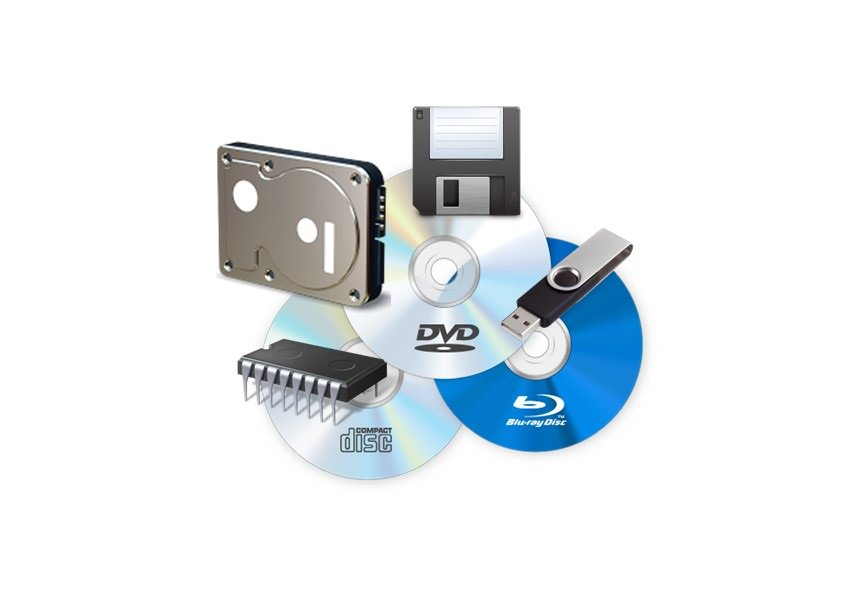
\includegraphics[width=13cm]{Imagens/zolpm4P.jpg}
\caption{Alguns exemplos de dispositivos de armazenamento}
\end{figure}

\chapter{Classificação}
\label{chap.classificacao}

\paragraph*{}Os dispositivos de armazenamento podem ser agrupados em quatro grandes categorias:

\section{Memória principal ou secundária}
\label{sect.memoriaprinsec}

\paragraph*{}A memória principal é uma memória a que o processador pode aceder diretamente. Esta memória funciona como uma espécie de ponte para a secundária e sem ela o computador não pode funcionar. A sua função é conter a informação necessária para o processador num determinado momento, como por exemplo, programas em execução (ex.: memória \ac{ram}).

\paragraph*{}A memória secundária é usada para gravar uma grande quantidade de dados por um longo período de tempo. Não pode ser endereçada diretamente, pelo que a informação precisa de passar por uma memória principal antes de poder ser tratada pelo processador e armazenada. Não é propriamente necessária para o funcionamento do sistema (ex.: \ac{cd}, PEN drive).

\section{Memória volátil ou não volátil}
\label{sect.memoriavolnvol}

\paragraph*{}Uma memória é considerada volátil quando requer energia para manter a informação armazenada. Assim, os dados são armazenados de forma temporária (ex.: memória RAM).

\paragraph*{}Por sua vez, uma memória é não volátil quando consegue guardar todas as informações, mesmo quando não estiverem a receber alimentação elétrica. Desta maneira, os dados são armazenados de forma permanente (ex.: memória \ac{rom}).

\newpage

\section{Dispositivo magnético, ótico ou eletrónico}
\label{sect.dispmagoticeletr}

\paragraph*{}Num dispositivo de armazenamento por meio magnético, a leitura e gravação das informações dá-se pela manipulação de dipolos magnéticos presentes na superfície do dispositivo magnético. No processo de gravação, a cabeça da leitura e gravação do dispositivo gera um campo magnético que magnetiza os dipolos magnéticos, representando assim dígitos binários (0 e 1 bits) de acordo com a polaridade utilizada (ex.: disquete). 

\paragraph*{}Os dispositivos de armazenamento por meio ótico utilizam processos de gravação a laser e são os mais utilizados para o armazenamento de filmes, música, etc. Além disso, também são muito utilizados para o armazenamento de informações e programas, sendo especialmente utilizados para a instalação de software no computador (ex.: \ac{cd}).

\paragraph*{}Um dispositivo de armazenamento por meio eletrónico, também conhecido como memória de estado sólido, é distinguido por não possuir partes móveis, apenas circuitos eletrónicos que não precisam de se movimentar para ler ou gravar informações, oferecendo um tempo de acesso muito menor que os outros tipos de dispositivos. (ex.: cartões de memória, PEN drives).

\section{Dispositivo removível ou não removível}
\label{sect.dispremovnremv}

\paragraph*{}Tal como a própria classificação indica, um dispositivo removível é aquele que o usuário pode retirar do computador, podendo assim transportar dados de um sistema informático para outro (ex.: \ac{dvd}, PEN drive).

\paragraph*{}Já um dispositivo não removível é aquele cuja remoção já não é possível por meios "normais", mas continua a ser possível retirá-lo do sistema, como é óbvio (ex.: \ac{hd}, memória \ac{ram}).

\chapter{Exemplos}
\label{chap.exemplos}
\paragraph*{}Vamos agora apresentar alguns exemplos de dispositivos de armazenamento e falar sobre cada um individualmente, referindo as suas características, história/evolução, classificação, vantagens e desvantagens.

\newpage

\section{Disquete}
\label{sect.disquete}

\begin{itemize}
\item Memória secundária;
\item Memória não volátil (permanente);
\item Dispositivo magnético;
\item Dispositivo removível.
\end{itemize}

\paragraph*{}A disquete foi apresentada no ano de 1970. Por mais de duas décadas foi o principal sistema de gravação e o mais utilizado nesses 20 anos. Era utilizada para carregar na memória o sistema operativo e instalar outros softwares, mas também era, ao mesmo tempo, o principal sistema de transferência de dados entre computadores.

\begin{figure}[H]
\center
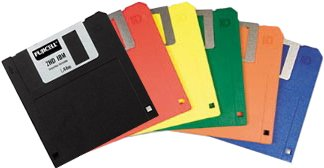
\includegraphics[width=5cm]{Imagens/disquetes.jpg}
\caption{Disquetes}
\end{figure}

\paragraph*{}Tinha uma capacidade total de cerca de 80 \ac{kb} (apenas 81920 bytes) e só posteriormente apareceram muitos outros modelos com diferentes capacidades. A mais vulgar é a de capacidade de 1.44 \ac{mb}. 

\paragraph*{}Está atualmente em desuso, pois foi substítuida por dispositivos de  armazenamento com capacidades imensamente maiores, como o CD, PEN drives, cartões de memória, discos externos, etc. dos quais falaremos a seguir.

\begin{figure}[H]
\center
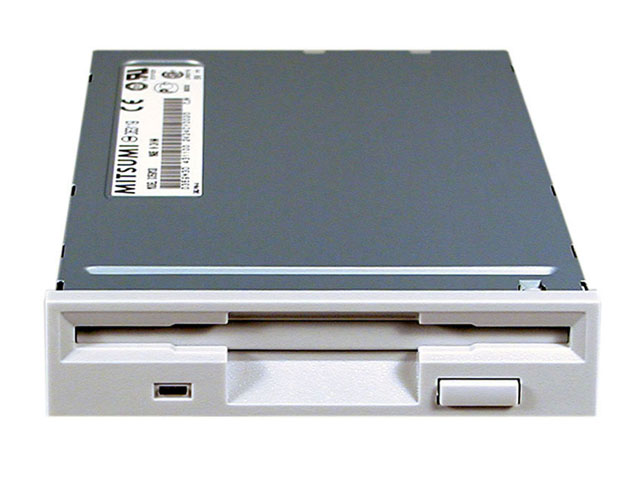
\includegraphics[width=5cm]{Imagens/leitor_disquete.jpg}
\caption{Leitor de disquetes}
\end{figure}

\newpage

\section{CD}
\label{sect.cd}

\begin{itemize}
\item Memória secundária;
\item Memória não volátil (permanente);
\item Dispositivo ótico;
\item Dispositivo removível.
\end{itemize}

O \ac{cd} foi inventado em 1979 e comercializado a partir de 1982. Este formato foi originalmente desenvolvido com o objetivo de armazenar e reproduzir apenas música, mas hoje em dia é também um dos mais populares meios de armazenamento de dados, continuando a ser ainda muito utilizado no que toca à área da música. 

\begin{figure}[H]
\center
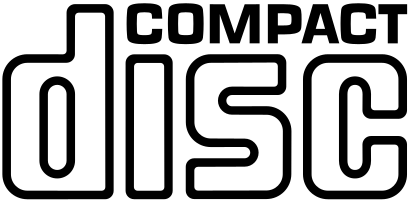
\includegraphics[width=1cm]{Imagens/cd_logo.png}
\end{figure}

\begin{figure}[H]
\center
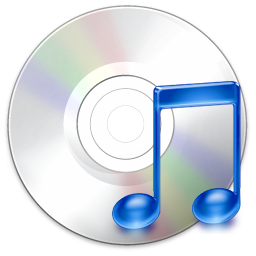
\includegraphics[width=5.5cm]{Imagens/cd.png}
\caption{\ac{cd}}
\end{figure}

\paragraph*{}Geralmente, os mais comuns têm uma capacidade de aproximadamente 700 \ac{mb} (o equivalente a 80 minutos) mas, no entanto, existem várias outras capacidades de armazenamento, dependendo do tipo de \ac{cd} a considerar.

\begin{figure}[H]
\center
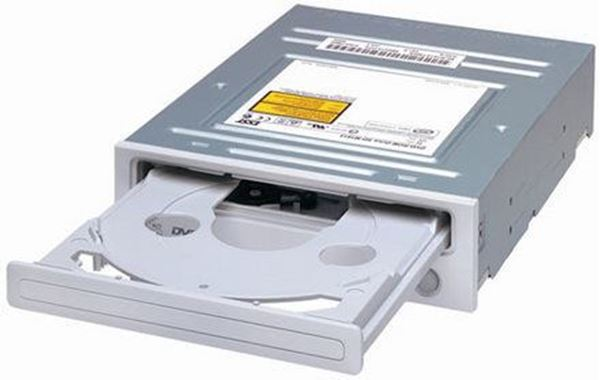
\includegraphics[width=5.5cm]{Imagens/leitor_cd.jpeg}
\caption{Leitor de \ac{cd}}
\end{figure}

\subsection{Tipos de CD}

\vspace*{7mm}

\subsubsection{CD-ROM} 
\paragraph*{}O Compact Disc - Read Only Memory (CD-ROM) é gravado uma única vez pelo seu fabricante. Após essa gravação, serve apenas para leitura e o seu conteúdo não pode ser apagado ou alterado, pois encontra-se protegido contra escrita. É muito utilizado para distribuição e instalação de software.

\begin{figure}[H]
\center
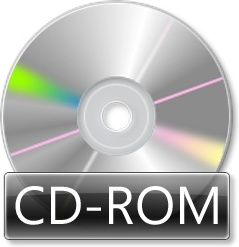
\includegraphics[width=1.5cm]{Imagens/cd-rom.jpg}
\caption{CD-ROM}
\end{figure}

\subsubsection{CD-R} 
\paragraph*{}O Compact Disc - Recordable (CD-R) só aceita uma única gravação e, após isso, os seus dados podem ser apagados mas o espaço usado não é recuperado, o que impossibilita outra gravação. É um dos tipos de \ac{cd} que tem maior aceitação nos mais diversos aparelhos. É a melhor opção para a gravação de músicas, pois é aceite por todos os leitores de \ac{cd}.

\begin{figure}[H]
\center
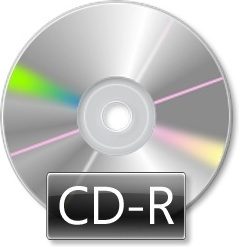
\includegraphics[width=1.5cm]{Imagens/cd-r.jpg}
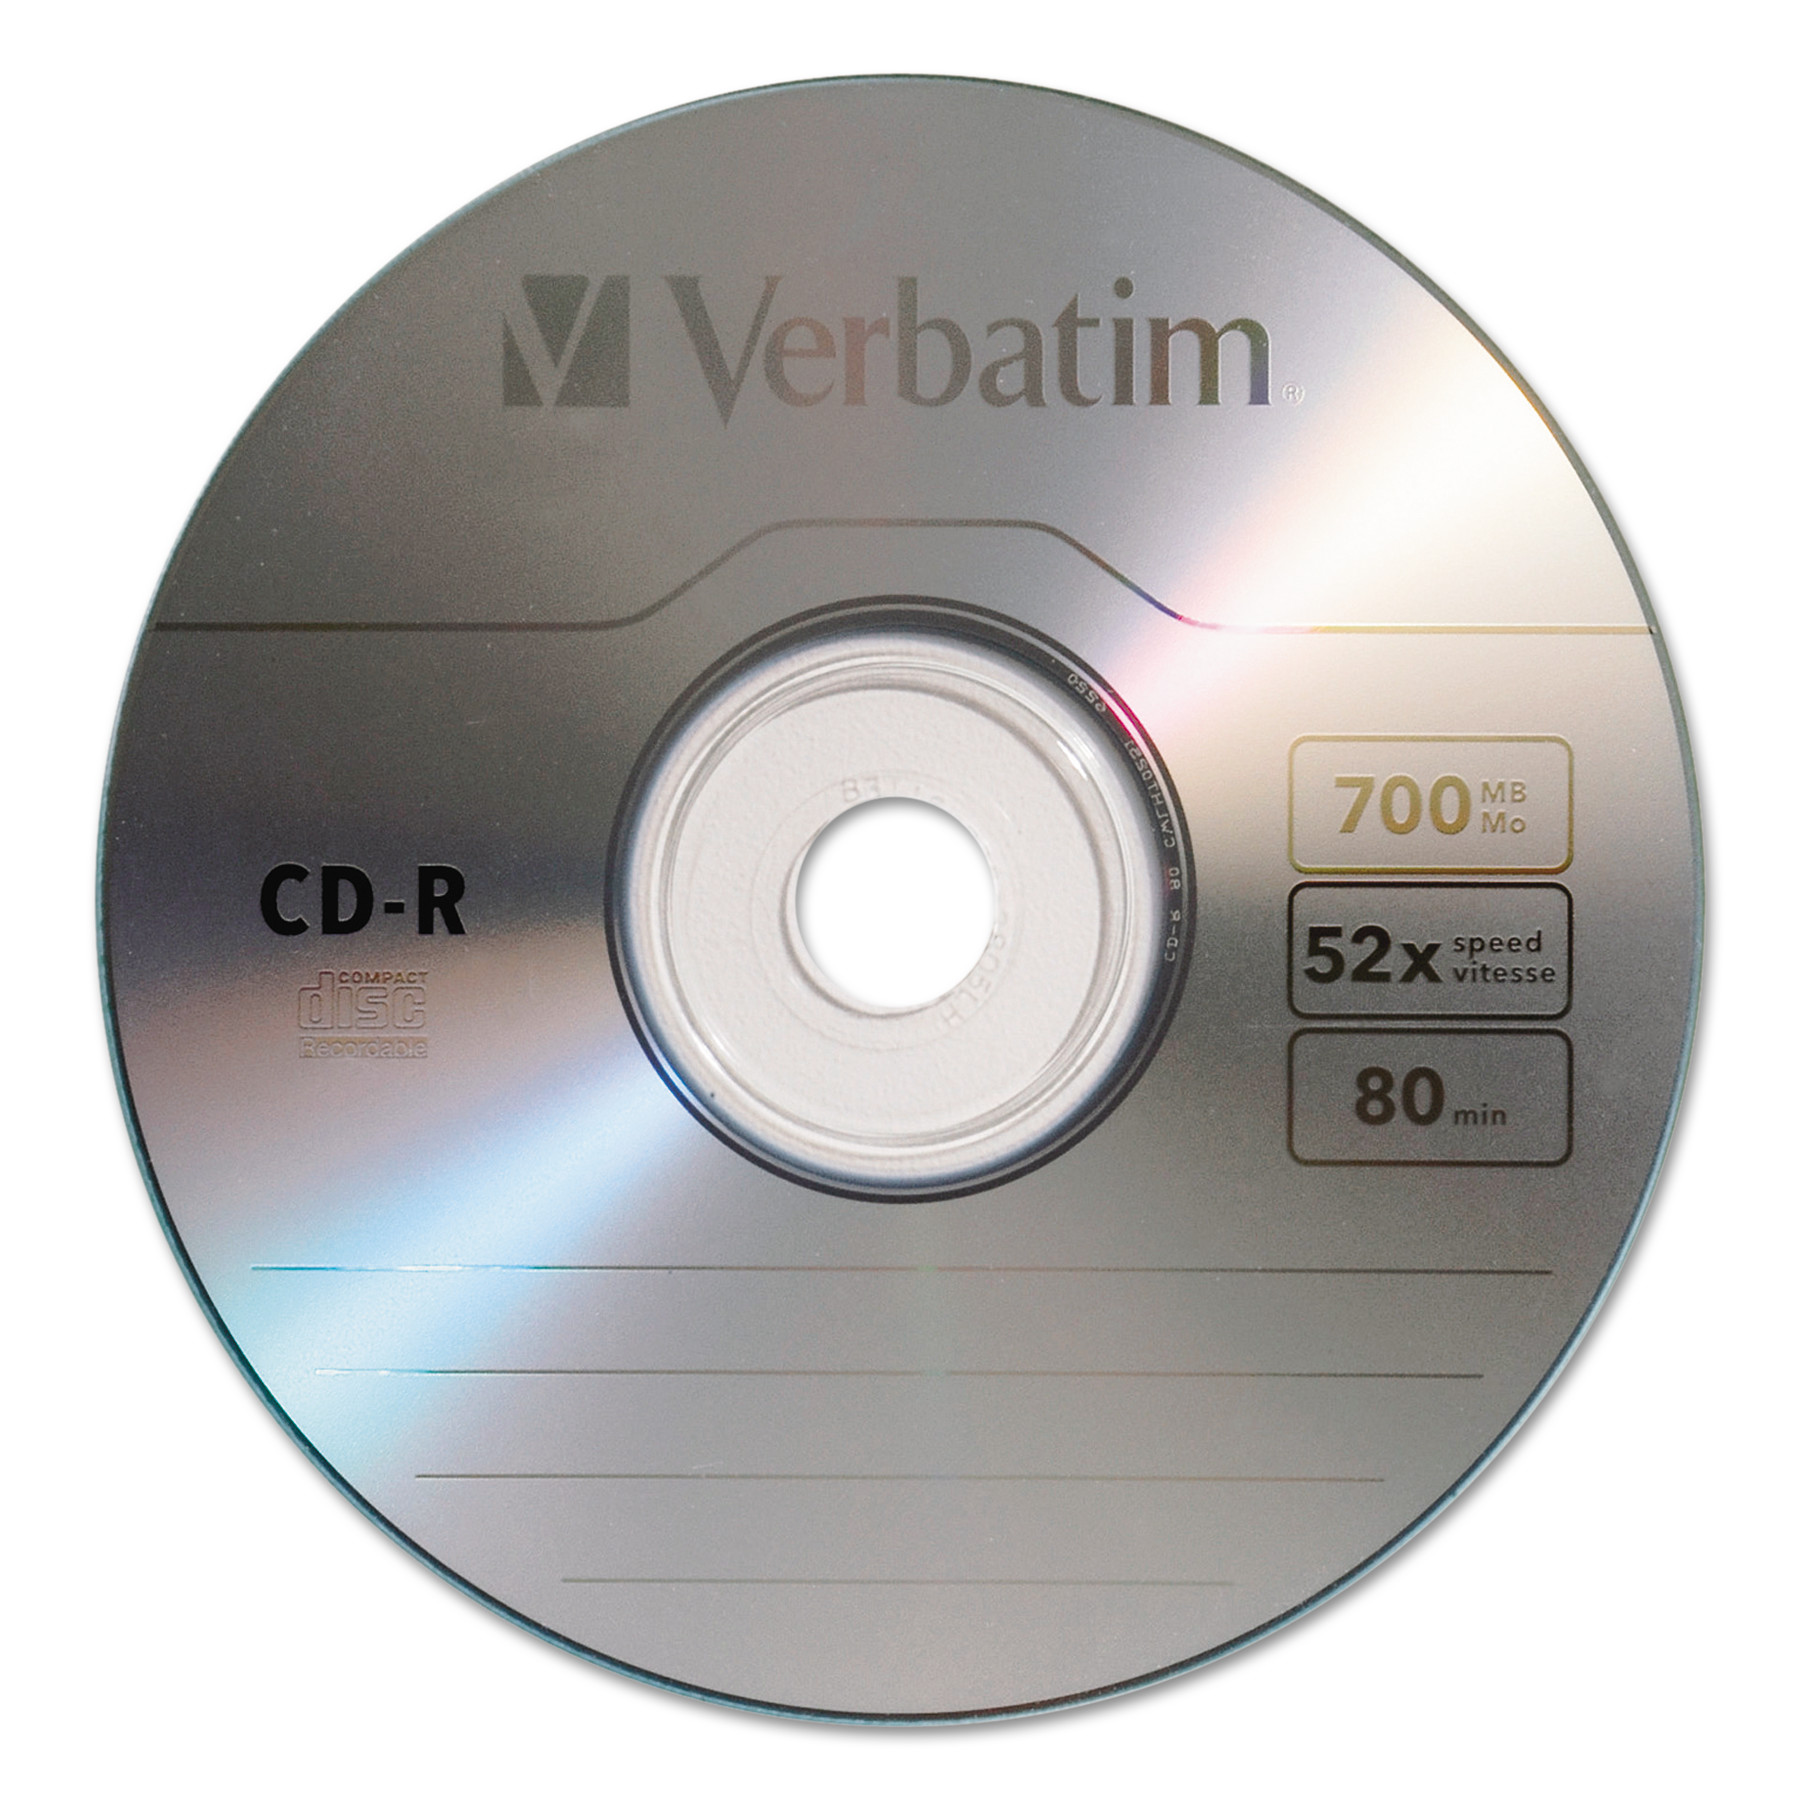
\includegraphics[width=3cm]{Imagens/cd-r-ex.jpeg}
\caption{CD-R}
\end{figure}

\subsubsection{CD-RW} 
\paragraph*{}O Compact Disc - ReWritable (CD-RW) permite a gravação e a regravação de dados até, aproximadamente, mil vezes. A maioria dos leitores de \ac{cd} recentes são totalmente compatíveis com CD-RW.

\begin{figure}[H]
\center
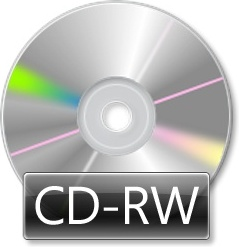
\includegraphics[width=1.5cm]{Imagens/cd-rw.jpg}
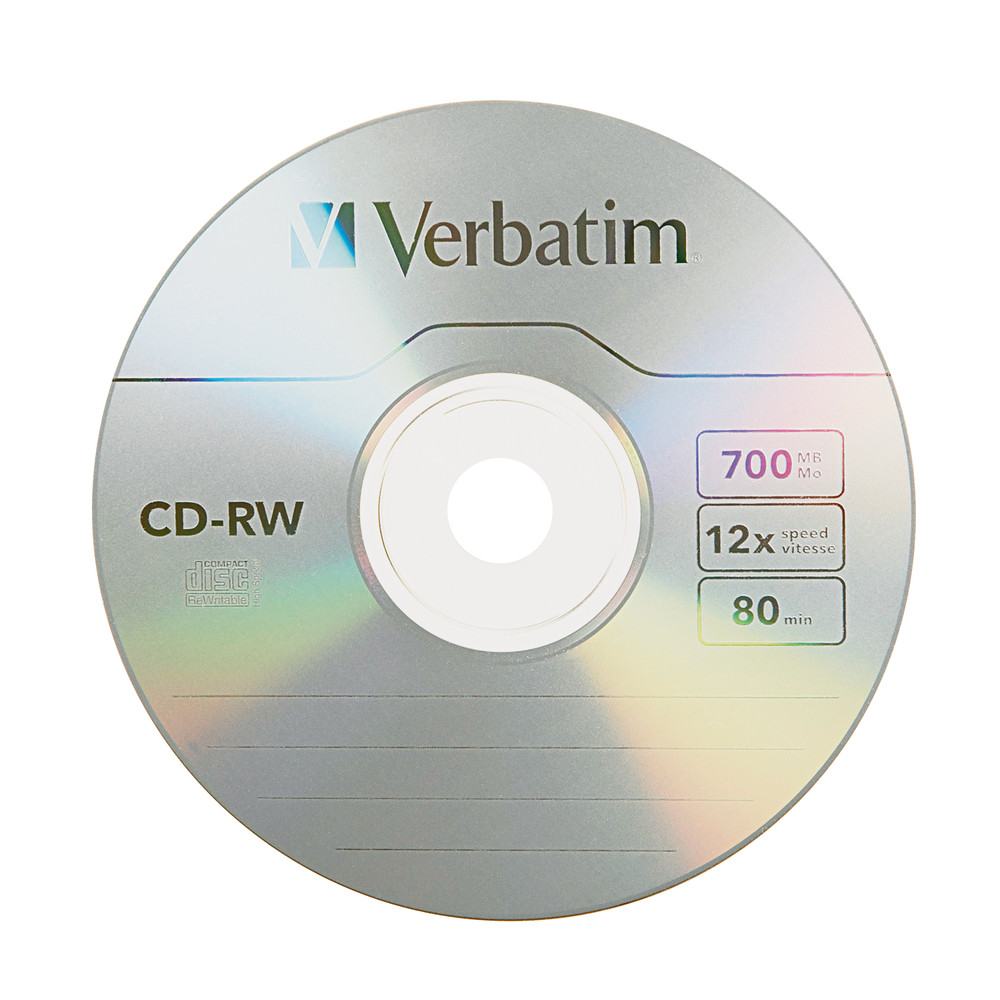
\includegraphics[width=3cm]{Imagens/cd-rw-ex.jpg}
\caption{CD-RW}
\end{figure}

\newpage

\section{DVD}
\label{sect.dvd}

\begin{itemize}
\item Memória secundária;
\item Memória não volátil (permanente);
\item Dispositivo ótico;
\item Dispositivo removível.
\end{itemize}

\paragraph*{}O \ac{dvd} veio substituir as fitas/cassetes de filme VHS e foi criado em 1995. Como é óbvio, o \ac{cd} não foi a invenção perfeita e não chegava, por exemplo, para gravar filmes\footnote{O espaço de um CD é apenas cerca de 14\% o espaço de um DVD}, pelo que foi necessário desenvolver este outro dispositivo com uma melhor compressão, um maior tamanho e uma melhor qualidade.
É atualmente ainda muito utilizado, principalmente no mercado de vídeo.

\begin{figure}[H]
\center
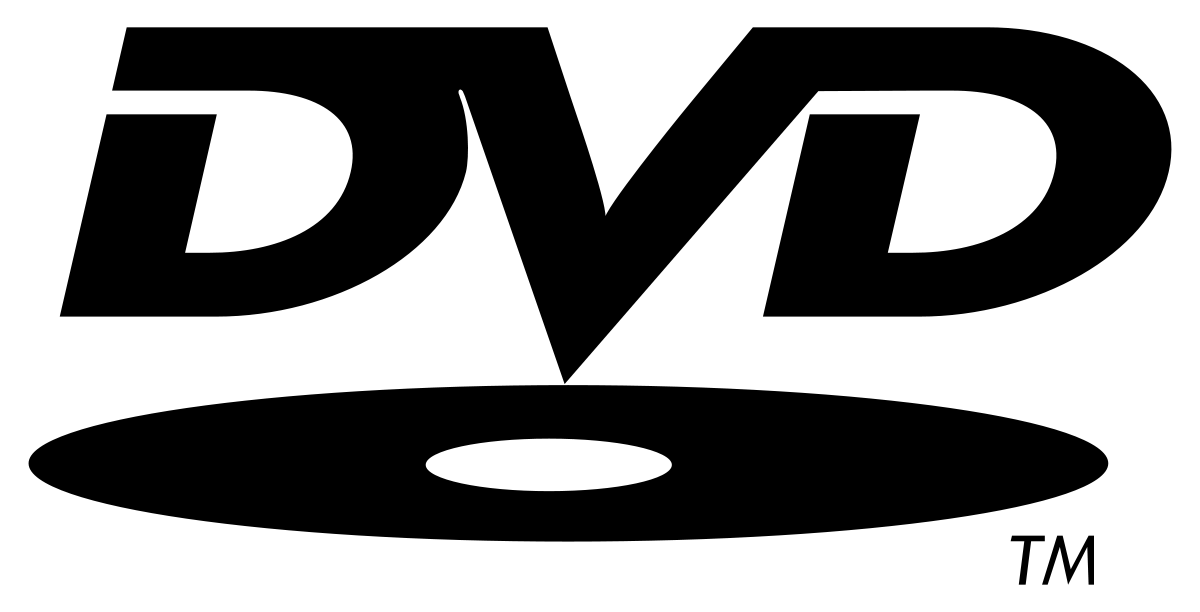
\includegraphics[width=3.5cm]{Imagens/dvd_logo.png}
\end{figure}

\begin{figure}[H]
\center
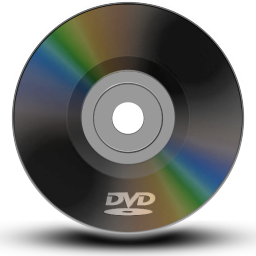
\includegraphics[width=5cm]{Imagens/dvd.png}
\caption{\ac{dvd}}
\end{figure}

\paragraph*{}Tinha uma capacidade de 4.7 \ac{gb}, podendo nos dias de hoje atingir os 17.08 \ac{gb}. Tal como o \ac{cd}, este dispositivo de armazenamento também é fabricado em diferentes tipos, muito idênticos aos tipos de \ac{cd}.

\begin{figure}[H]
\center
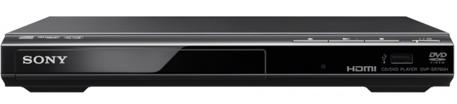
\includegraphics[width=7cm]{Imagens/leitor_dvd.jpg}
\caption{Leitor de \ac{dvd}}
\end{figure}

\vspace*{5mm}

\subsection{Tipos de DVD}

\vspace*{8mm}

\subsubsection{DVD-ROM} 
\paragraph*{}O Digital Video Disc - Read Only Memory (DVD-ROM) não permite a gravação de dados. Esta já vem feita de fábrica e é impossível gravar/modificar/apagar os dados nele contidos, pois encontram-se protegidos contra escrita.

\begin{figure}[H]
\center

\includegraphics[width=2cm]{Imagens/dvd-rom.png}
\caption{DVD-ROM}
\end{figure}

\subsubsection{DVD-R} 
\paragraph*{}O Digital Video Disc - Recordable (DVD-R) permite a gravação de dados apenas uma vez.

\begin{figure}[H]
\center
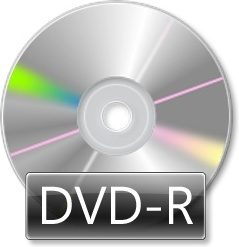
\includegraphics[width=2cm]{Imagens/dvd-r.jpg}
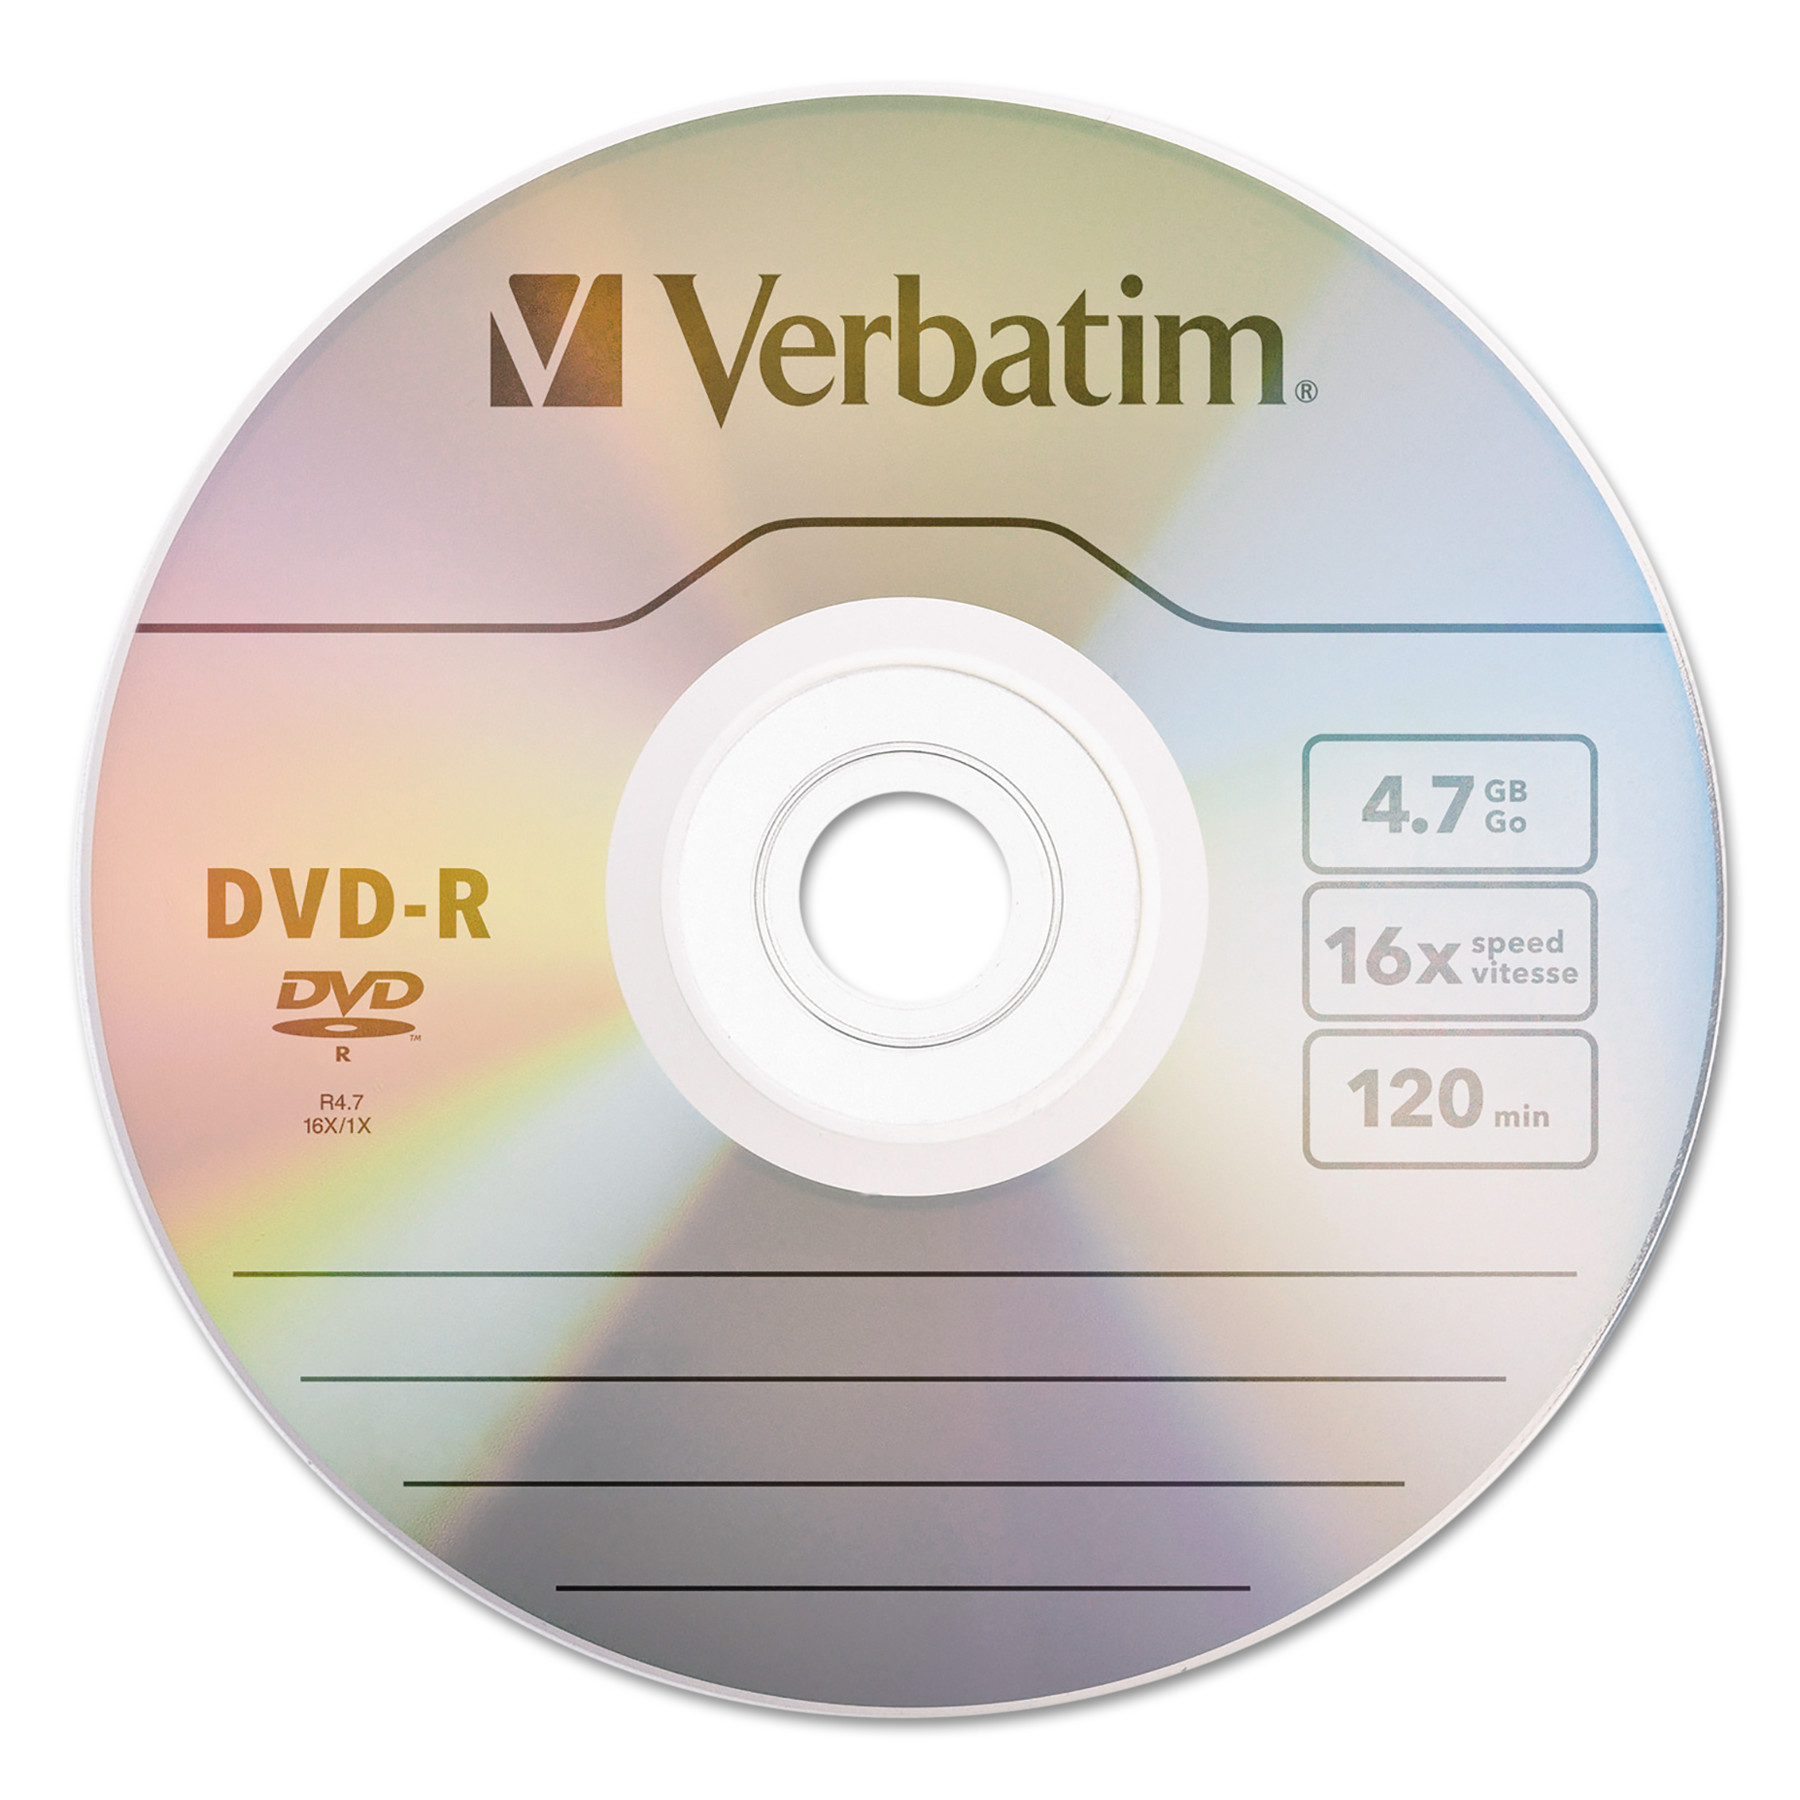
\includegraphics[width=6cm]{Imagens/dvd-r-ex.jpeg}
\caption{DVD-R}
\end{figure}

\newpage

\subsubsection{DVD-RW} 
\paragraph*{}O Digital Video Disc - ReWritable (DVD-RW) permite a gravação e a regravação de dados. É frequentemente utilizado para fazer cópias de segurança de dados em computadores pessoais.

\begin{figure}[H]
\center
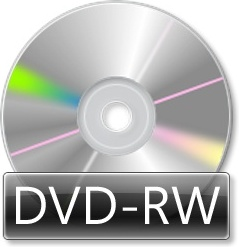
\includegraphics[width=2cm]{Imagens/dvd-rw.jpg}
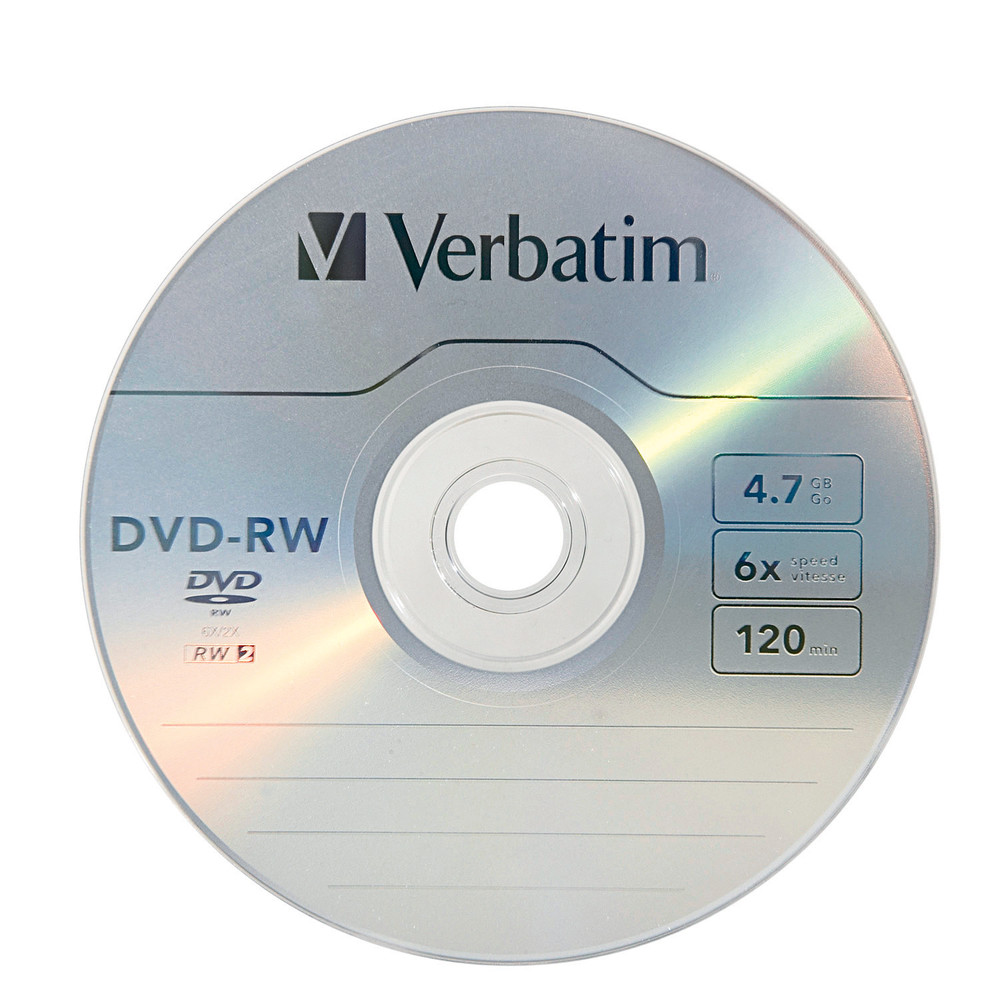
\includegraphics[width=6cm]{Imagens/dvd-rw-ex.jpg}
\caption{DVD-RW}
\end{figure}

\subsubsection{DVD-RAM} 
\paragraph*{}O Digital Video Disc - Random Access Memory (DVD-RAM) permite a gravação e regravação de dados de forma semelhante aos DVD-RW, mas mais rapidamente do que estes. 

\begin{figure}[H]
\center
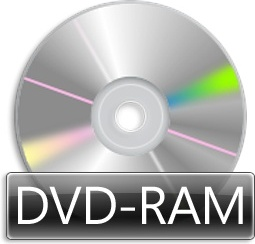
\includegraphics[width=2cm]{Imagens/dvd-ram.jpg}
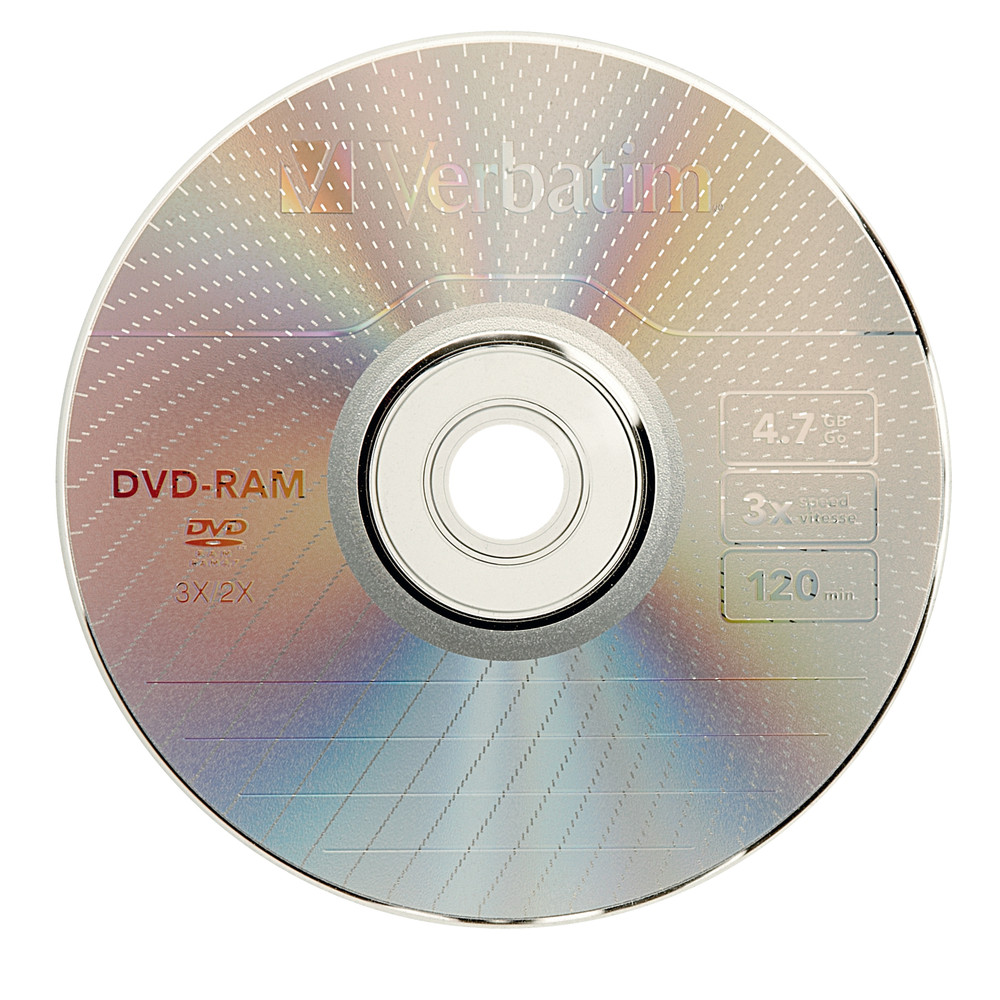
\includegraphics[width=6cm]{Imagens/dvd-ram-ex.jpg}
\caption{DVD-RAM}
\end{figure}

\newpage

\section{Disco Blu-ray}
\label{sect.bluray}

\begin{itemize}
\item Memória secundária;
\item Memória não volátil (permanente);
\item Dispositivo ótico;
\item Dispositivo removível.
\end{itemize}

\paragraph*{}O disco Blu-ray é uma alternativa ao \ac{dvd} e é utilizado no armazenamento de dados de alta densidade e vídeo de alta definição (Full HD 1080p). Requer uma televisão LCD/LED Full HD para que todo o seu potencial possa ser explorado.

\begin{figure}[H]
\center

\includegraphics[width=4cm]{Imagens/bluray_logo.png}
\end{figure}

\begin{figure}[H]
\center
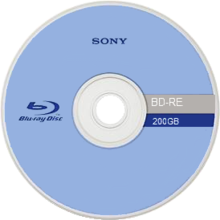
\includegraphics[width=5cm]{Imagens/bluray.png}
\caption{Disco Blu-ray}
\end{figure}

\paragraph*{}Os discos Blu-ray têm geralmente a capacidade para 25/50 \ac{gb} mas os mais caros podem chegar aos 200 \ac{gb}.

\begin{figure}[H]
\center
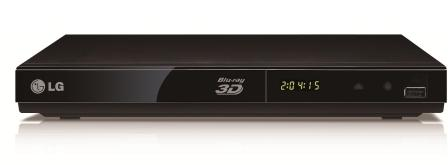
\includegraphics[width=8cm]{Imagens/leitor_bluray.jpg}
\caption{Leitor de discos Blu-ray}
\end{figure}

\newpage

\section{Cartão de Memória}
\label{sect.cartaomemoria}

\begin{itemize}
\item Memória secundária;
\item Memória não volátil (permanente);
\item Dispositivo eletrónico;
\item Dispositivo removível.
\end{itemize}

\paragraph*{}Os cartões de memória servem para aumentar a capacidade do aparelho em que se colocam e assim armazenar mais dados como texto, fotos, vídeos, músicas e outros documentos pessoais.
Estes são usados em diferentes tipos de dispositivos de hardware como, por exemplo, dispositivos GPS, cameras fotográficas digitais, telemóveis e leitores de MP3. 
\paragraph*{}Há uma variedade enorme de cartões de memória para o utilizador escolher, desde 128 \ac{mb} até 2 \ac{tb}. Os mais usados atualmente são os \ac{sd}, os \ac{sdhc} ou ainda os \ac{sdxc} devido às suas rápidas velocidades de gravação/leitura e às suas monstruosas capacidades de armazenamento.

\subsection{Tipos de cartões de memória}

\paragraph*{}Segue-se uma tabela com alguns dos tipos de cartões de memória mais comuns e mais utilizados:

\vspace{8mm}

\begin{tabular}{|c|c|c|c|}
\hline
\large\textbf{Imagem} & \large\textbf{Nome} & \large\textbf{Capacidade} & \large\textbf{Utilização}\\\hline
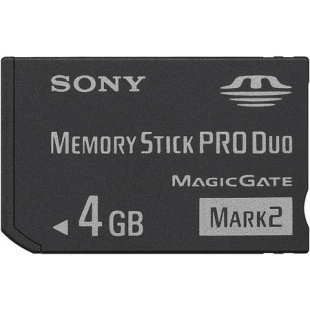
\includegraphics[scale=0.2]{Imagens/4-5-1.png} & Memory Stick & 256\ac{mb} até 32\ac{gb} & Cameras digitais Sony e PSP’s\\\hline
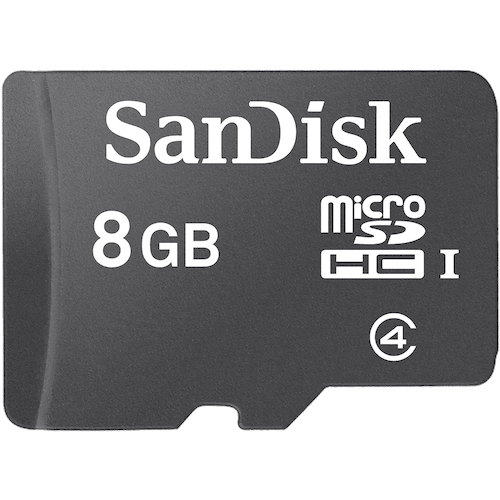
\includegraphics[scale=0.1]{Imagens/4-5-2.png} & Micro \ac{sd} & 128\ac{mb} até 256\ac{gb} & Telemóveis, dispositivos GPS, etc.\\\hline 
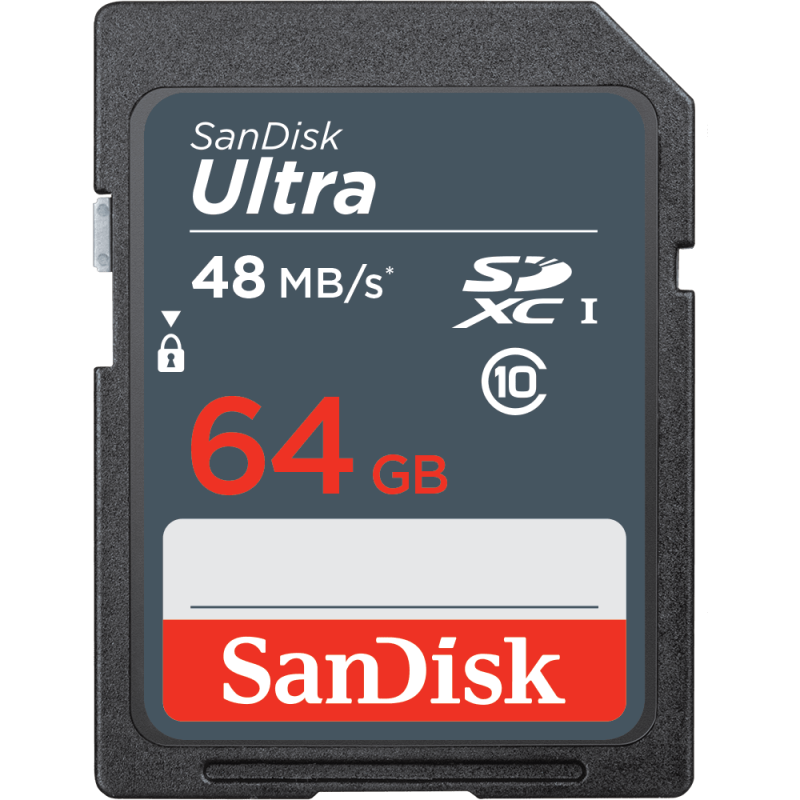
\includegraphics[scale=0.07]{Imagens/4-5-3-1.png} & \ac{sd} / \ac{sdhc} / \ac{sdxc} & 128\ac{mb} até 2\ac{tb} & Tablets, cameras digitais, etc. \\\hline
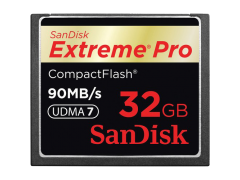
\includegraphics[scale=0.3]{Imagens/4-5-4.png} & Compact Flash & 8\ac{mb} até 64\ac{gb} & Cameras digitais profissionais\\\hline 
\end{tabular}

\newpage

\section{PEN Drive}
\label{sect.pen}

\begin{itemize}
\item Memória secundária;
\item Memória não volátil (permanente);
\item Dispositivo eletrónico;
\item Dispositivo removível.
\end{itemize}

\paragraph*{}As PEN drives apareceram no mercado em 2000 e revolucionaram a forma de transporte de ficheiros por serem compactas e de ligação fácil através das portas \ac{usb}, não necessitando instalação prévia de qualquer software.

\begin{figure}[H]
\center
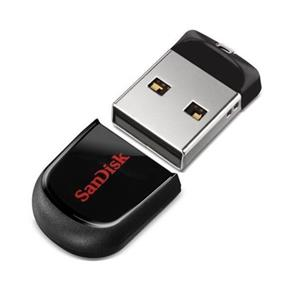
\includegraphics[width=4.5cm]{Imagens/pen.jpg}
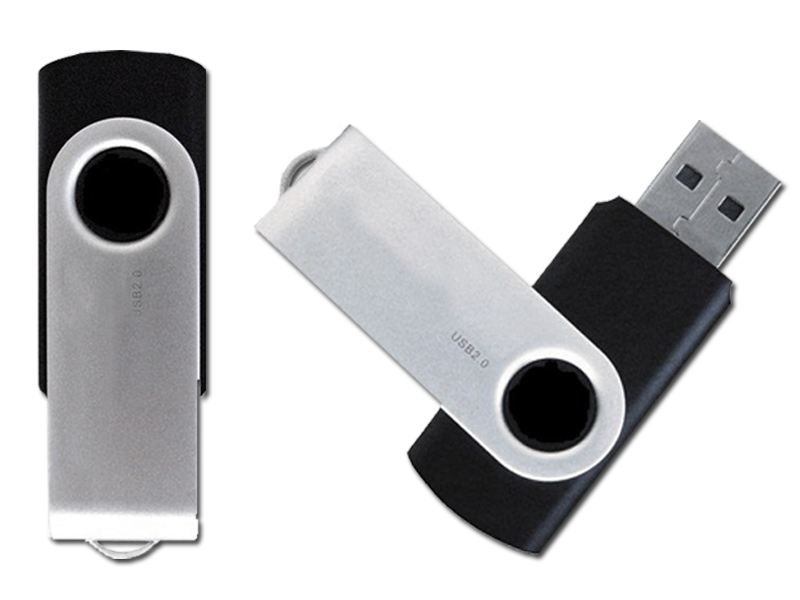
\includegraphics[width=6cm]{Imagens/pen2.png}
\caption{PEN Drives}
\end{figure}

\paragraph*{}Atualmente, a sua capacidade de armazenamento varia de 64 \ac{mb} a 1 \ac{tb}. É uma das formas mais populares de transporte e armazenamento de dados da atualidade e permanecerá assim por muito tempo, visto a quantidade de vantagens que estes dispositivos oferecem face a outros dispositivos de armazenamento portáteis.

\begin{figure}[H]
\center
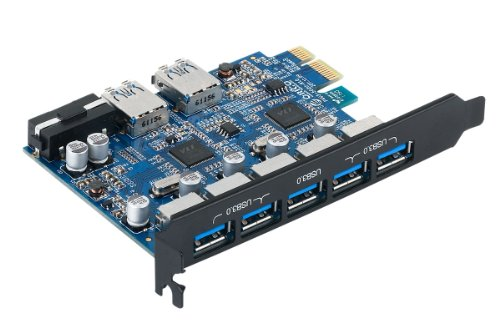
\includegraphics[width=9cm]{Imagens/porta_usb.jpg}
\caption{Portas \ac{usb}}
\end{figure}

\section{Disco HDD}
\label{sect.hdd}

\begin{itemize}
\item Memória secundária;
\item Memória não volátil (permanente);
\item Dispositivo magnético e eletrónico;
\item Dispositivo não removível.
\end{itemize}

\paragraph*{}Quando falamos em \ac{hdd} referimo-nos ao disco rígido tradicional que equipa a maioria dos computadores. Trata-se de um sistema de armazenamento de alta capacidade constituído por pratos metálicos que rodam a alta velocidade e que possuem uma cobertura magnética. Com o uso de uma cabeça de leitura, igualmente móvel, os dados guardados são acedidos. Mas naturalmente todo este sistema está normalmente invisível ao utilizador uma vez que o disco é fornecido no interior de uma caixa metálica fechada (e que se torna necessária pois um simples grão de pó poderia criar problema ao sistema). É um dos dispositivos de armazenamento de informações indispensável ao funcionamento do computador. Atualmente os \ac{hdd} rondam os 3 \ac{tb} de capacidade máxima.

\begin{figure}[H]
\center
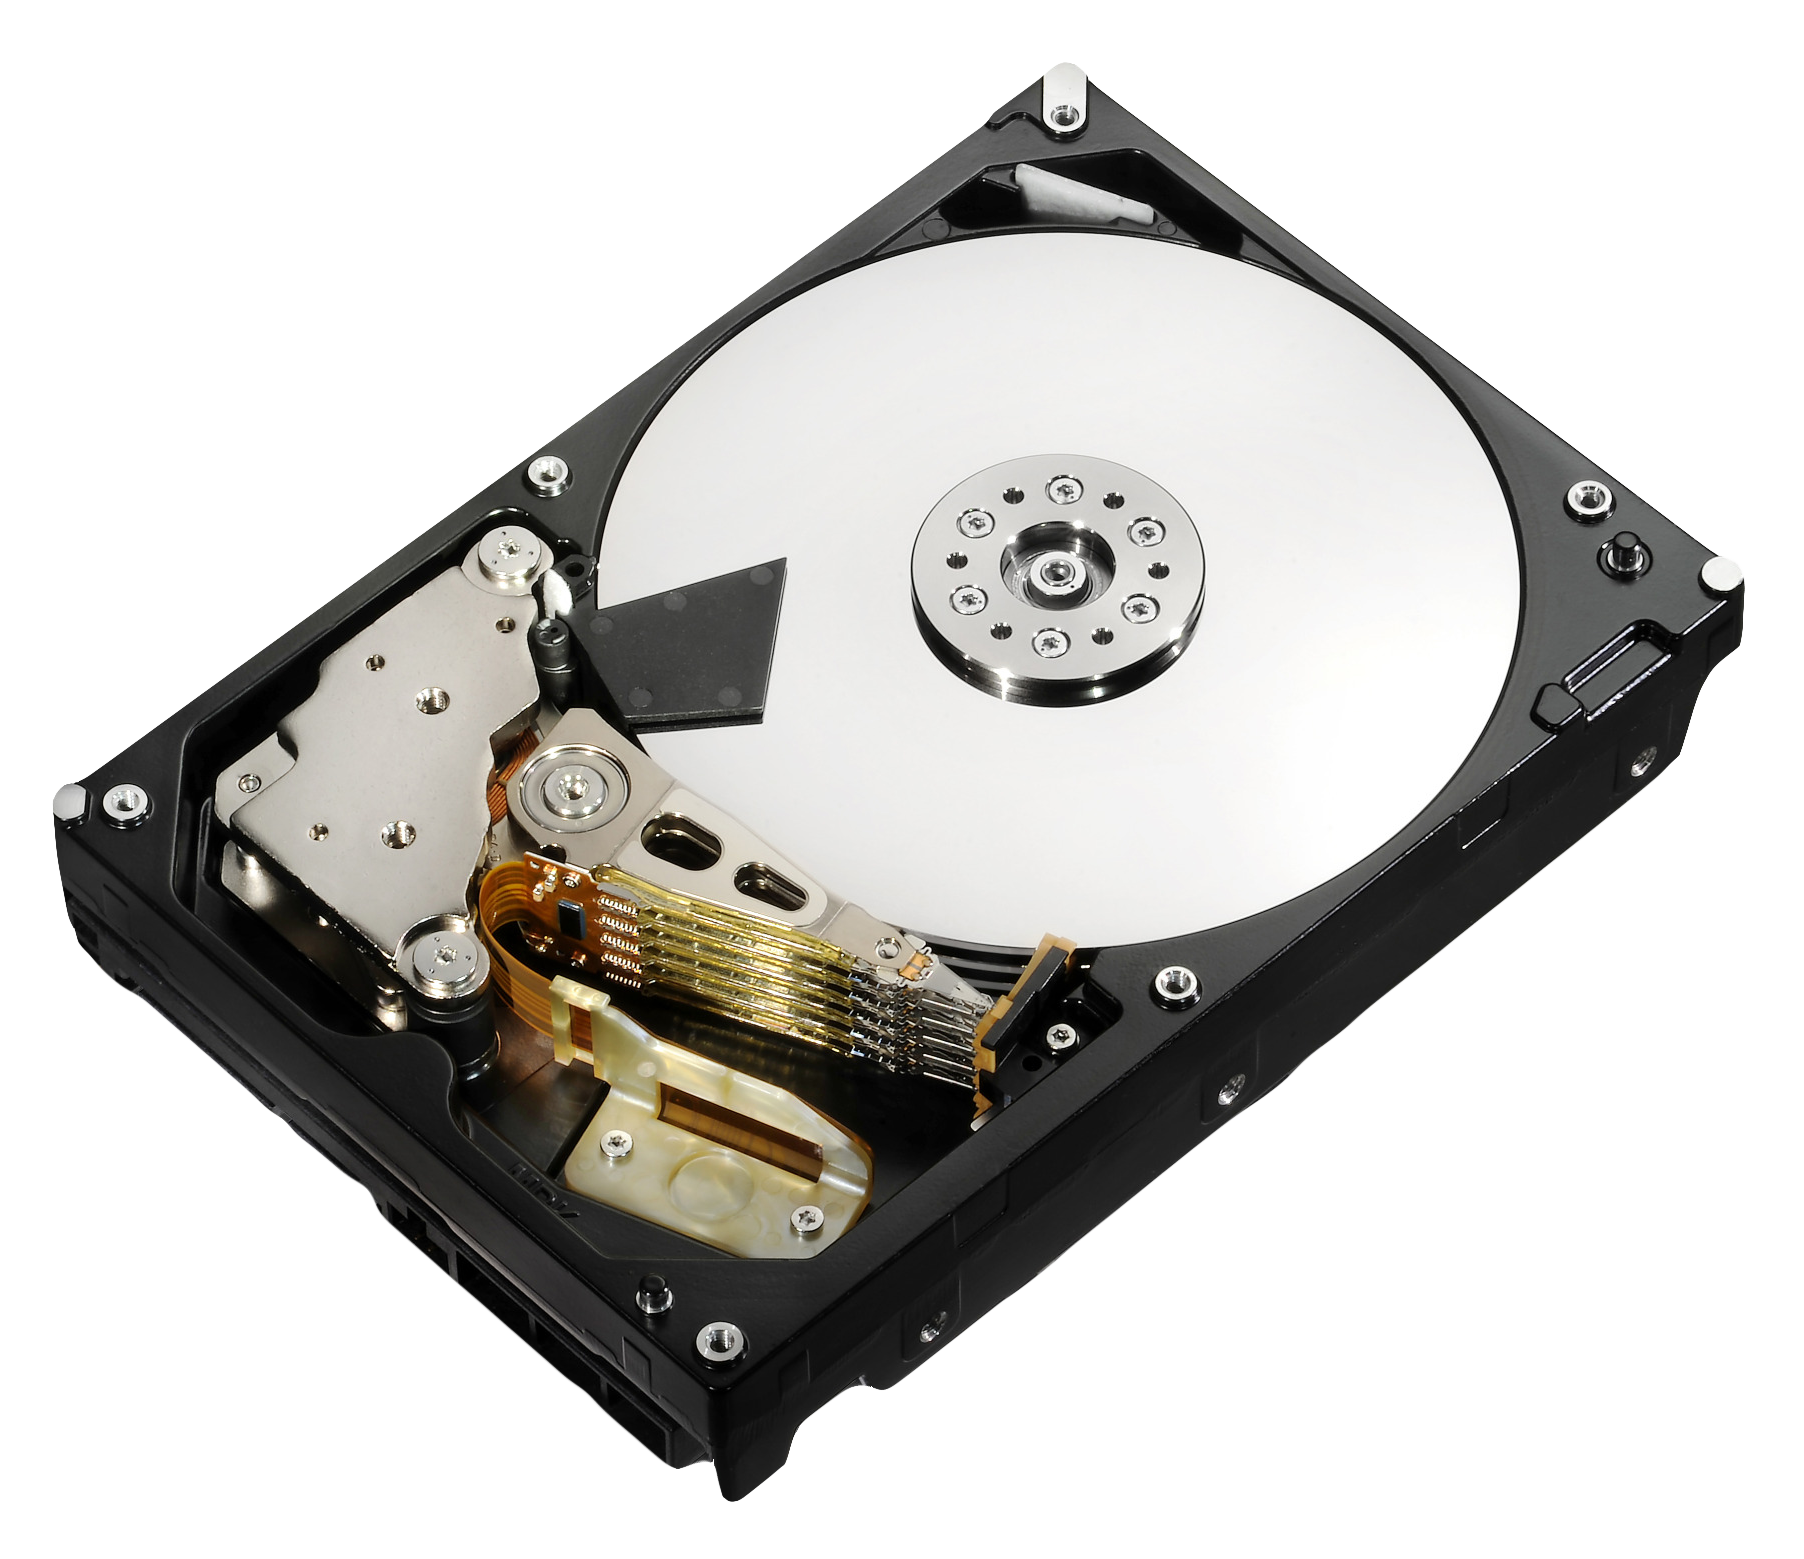
\includegraphics[width=9cm]{Imagens/imagemdehdd.png}
\caption{Disco \ac{hdd}}
\end{figure}

\newpage

\section{Disco SSD}
\label{sect.ssd}

\begin{itemize}
\item Memória secundária;
\item Memória não volátil (permanente);
\item Dispositivo eletrónico;
\item Dispositivo não removível.
\end{itemize}

\paragraph*{} \ac{ssd} é um sistema cujo método de funcionamento, na parte que toca ao utilizador, é exatamente idêntico ao do \ac{hdd}, mas já no que toca ao seu interior todo o sistema de pratos rotativos e cabeças de leitura é substituído por chips de memória flash, ao estilo da usada nas Pen drives. Esta memória consegue manter os dados armazenados mesmo sem a presença de energia, tal como a das pen drives. A grande diferença aqui está na qualidade, velocidade e fiabilidade destas memórias que em nada se comparam à usada nas pens, e que tornam estes sistemas muito mais caros. E tal como nos discos rígidos, estes \ac{ssd}’s são fornecidos em caixas metálicas com formatos semelhantes aos do \ac{hdd} , quanto mais não seja porque fisicamente são colocados nas caixas nos mesmos locais dos discos rígidos tradicionais.

\begin{figure}[H]
\center
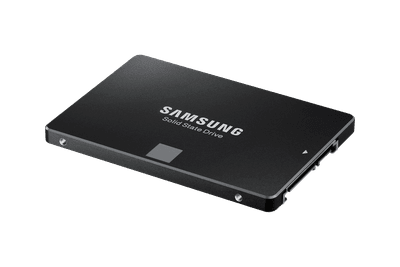
\includegraphics[width=6cm]{Imagens/imagemssd.png}
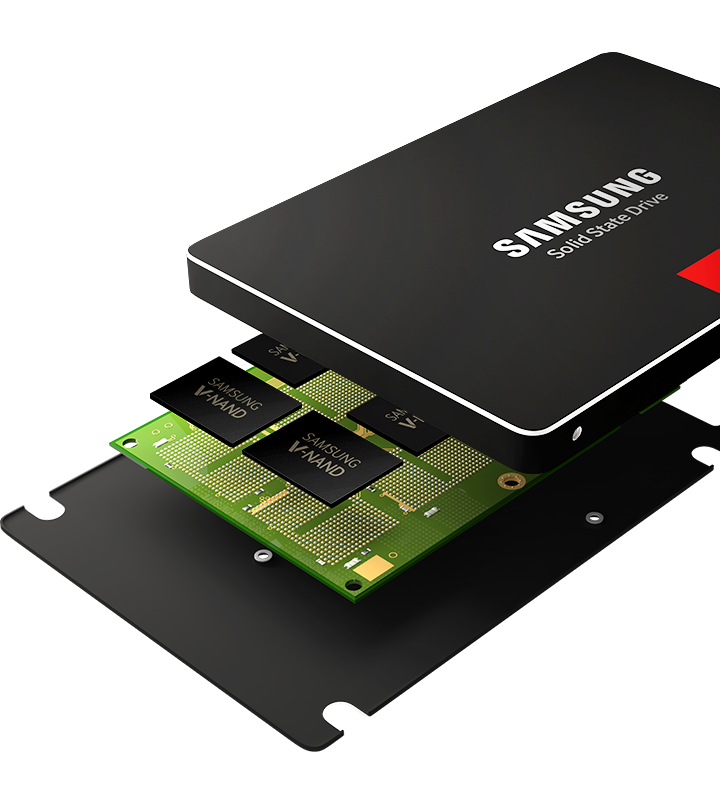
\includegraphics[width=5cm]{Imagens/discossd.png}
\caption{Disco \ac{ssd}}
\end{figure}

\newpage

\paragraph*{} Falaremos agora das diferenças, vantagens e desvantagens de cada um.

\subsection{Diferenças entre disco \ac{hdd} e \ac{ssd}}

\subsubsection*{Preço}

Como referido anteriormente, uma das diferenças entre os dois sistemas é o preço. É que um disco \ac{ssd} é bastante mais caro que um \ac{hdd} tradicional, mas essa é uma situação compensada por outras que abordaremos de seguida, e que tornam os \ac{ssd} atrativos.
Ao passo que um \ac{hdd} normal de 1 \ac{tb} custará em média cerca de 100 a 120 euros, já para um \ac{ssd} um disco de 1 \ac{tb} irá rondar os 1000 euros. É um preço de 10 cêntimos por Megabyte num disco \ac{hdd} e cerca de 1 Euro por Megabyte num \ac{ssd}. 
Sendo assim, para que queremos um \ac{ssd}? A resposta são as diferenças que seguem.

\subsubsection*{Velocidade}

A velocidade é o motivo pelo qual os \ac{ssd} existem. Diga-se que um sistema equipado com um \ac{ssd} pode arrancar um computador em meros segundos uma vez que não há os constrangimentos dos tradicionais \ac{hdd}. Os pratos não necessitam de acelerar, não existem diferenças de velocidade entre as pistas externas e internas do prato (a velocidade angular é constante mas dado que a densidade de gravação é constante, as pistas exteriores percorrem mais espaço no mesmo tempo), e acima de tudo a fragmentação do disco.
É que devido à forma como os discos funcionam a informação é colocada sequencialmente em forma de blocos. Quando alguns blocos são apagados, os espaços vazios são posteriormente preenchidos com nova informação, e quando os blocos necessários são superiores aos disponíveis o ficheiro fragmenta-se em partes espalhadas pelo disco, o que leva a maior tempo de pesquisa e leitura.
Os \ac{ssd} possuem o mesmo problema, mas dado que não há a necessidade de pesquisa física na superfície do disco pelas partes e os tempos de acesso à memória são, comparativamente, infinitamente menores, o problema assume menores proporções.
Mas a grande diferença entre os sistemas não é só essa, e há outro fator que os distingue de forma notória.

\newpage

\subsubsection*{Durabilidade}

No que toca à fiabilidade dos dados em caso de queda ou choque violento, os \ac{ssd}’s revelam-se superiores ao não possuírem partes móveis. Aliás um simples toque no prato da cabeça do \ac{hdd} poderá ser desastroso, e convém não esquecer que ela trabalha a meros mícrons de distância da camada magnética. É por esse motivo que os discos rígidos recolhem a cabeça de leitura quando são desativados.
Atualmente os \ac{ssd}’s são quase todos capazes de mais de 100 mil ciclos de escrita, e o Windows 7 e Windows 8 acrescentaram a deteção automática de \ac{ssd}’s bem como comandos de escrita dedicados para este tipo de discos, o que diminui bastante o desgaste destes discos em utilização normal, permitindo uma maior longevidade.

\subsubsection*{Ruído}

Falando agora de uma última vantagem notória dos \ac{ssd}, a total ausência de ruído. É que dado não existirem peças móveis e a temperatura de funcionamento ser baixa o suficiente para uma dissipação passiva ser eficaz, o ruído gerado é zero.
A somar a todas estas vantagens, os discos \ac{ssd} têm ainda a vantagem de serem mais compactos, pelo que permitem que o computador no qual estão integrados seja mais fino e leve. E também o facto de consumirem menos energia reduzindo assim o consumo, permitindo uma maior poupança e duração da bateria.

\newpage

\section{Disco Externo}
\label{sect.externo}

\begin{itemize}
\item Memória secundária;
\item Memória não volátil (permanente);
\item Dispositivo eletrónico;
\item Dispositivo removível.
\end{itemize}

O disco rígido (muitas vezes chamado de \ac{hd}) é o dispositivo que armazena os dados existentes no computador. Todos os arquivos, fotos, programas, tudo, está guardado no \ac{hd}. Todos os \ac{hd}’s possuem um limite de memória, por isso, quando temos demasiados arquivos, é necessário libertar espaço, removendo os arquivos menos utilizados e colocando-os noutro lugar, no qual não haja risco de se perderem tais documentos, mas que também seja de fácil acesso. É aí que entra o \ac{hd} externo, que vai armazenar os dados de maneira segura para que possam ser utilizados sempre que necessário.
Sendo um equipamento com enorme capacidade de armazenamento de dados, um \ac{hd} externo pode chegar a ultrapassar o 40 \ac{tb} de memória, completamente portátil e fácil de usar. Atendendo à sua enorme capacidade de armazenamento, o \ac{hd} externo também tem maior capacidade e velocidade de acesso aos dados, chegando a ser melhor do que um portátil normal.
O seu tamanho reduzido torna os \ac{hd} externos na derradeira forma de transporte de dados em massa. 
São muito utilizados na atualidade no armazenamento de grandes quantidades de informação pela sua portabilidade o que facilita a movimentação desses dados entre vários computadores.

\paragraph{}
\paragraph{}
\paragraph{}

\begin{figure}[H]
\center
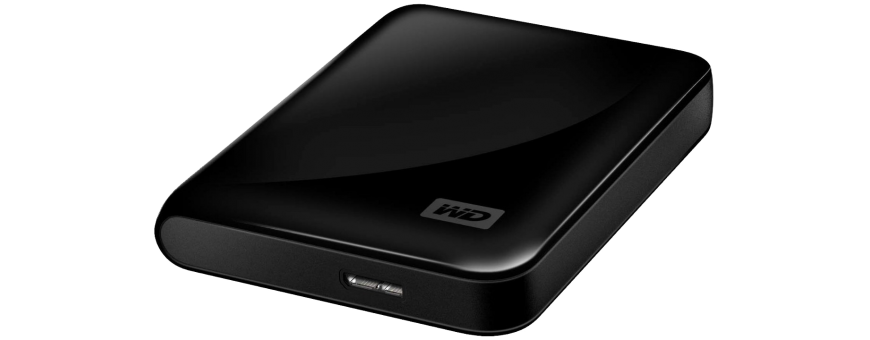
\includegraphics[width=7cm]{Imagens/discoexterno.png}
\caption{\ac{hd} externo}
\end{figure}

\newpage

\section{Memória RAM}
\label{sect.ram}

\begin{itemize}
\item Memória principal;
\item Memória volátil (temporária);
\item Dispositivo eletrónico;
\item Dispositivo não removível.
\end{itemize}

A memória \ac{ram} é um chip semelhante a um micro-processador, composto por milhões de transístores e condensadores. O condensador é uma peça capaz de armazenar eletrões. Quando o condensador está carregado, o sistema faz uma leitura com base em código binário. Essa leitura é feita de forma muito rápida, são muitas leituras em poucos milésimos de segundos. É assim que a memória \ac{ram} processa todas as ações executadas pelo utilizador. Esta memória é mantida por pulsos elétricos. 
Para simplificar a lógica por trás da função da memória \ac{ram}, é possível fazer uma analogia com uma mesa de estudos, onde se reúne todo o material necessário para realizar os trabalhos de casa: como canetas, lápis, cadernos e livros. Os materiais seriam os arquivos e a memória \ac{ram}, a mesa, onde tudo se reúne e o trabalho é feito.
Sendo assim, a memória \ac{ram} pode ser entendida como um espaço temporário de trabalho, pois, após a tarefa ser realizada, os arquivos (material de estudo) são retirados da memória (mesa) e mantidos no \ac{hd} (armário).
\subsubsection{Como funciona:}
Assim como a mesa, quanto maior a memória \ac{ram}, maior a sua capacidade de trabalho. Mas a capacidade da mesa é medida em área. Já a capacidade da memória \ac{ram}, mede-se pelo fluxo de bits suportados nas operações.
Ou seja, para se aceder a uma grande quantidade de memória no \ac{hd} de uma só vez, como muitos programas atuais exigem, é necessário uma grande quantidade de memória \ac{ram}. É de salientar que por mais memória que o \ac{hd} possua, é sempre necessária um certa quantidade de memória \ac{ram} pois sem ela a execução dos programas seria muito mais lenta.

\begin{figure}[H]
\center
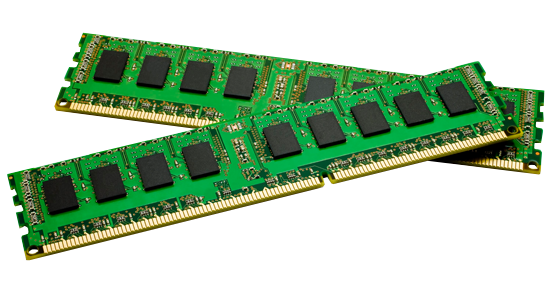
\includegraphics[width=7cm]{Imagens/ram.png}
\caption{Memória \ac{ram}}
\end{figure}

\newpage

\section{Memória ROM}
\label{sect.rom}

\begin{itemize}
\item Memória principal;
\item Memória não volátil (permanente);
\item Dispositivo eletrónico;
\item Dispositivo não removível.
\end{itemize}

A \ac{rom} é um tipo de memória em que os dados não se perdem quando o computador é desligado. 
A memória \ac{rom} permite apenas a leitura de dados, ou seja, não permite a gravação de dados, apenas se pode ver ou executar o seu conteúdo. São memórias cujo conteúdo é gravado permanentemente. Basicamente, essa é a função da memória \ac{rom}: oferecer dados apenas para leitura. Normalmente, a ROM é utilizada para armazenar firmwares, pequenos softwares que funcionam apenas no hardware para o qual foram desenvolvidos e que controlam as funções mais básicas do dispositivo.
Na \ac{rom} de uma calculadora, por exemplo, podemos encontrar as rotinas matemáticas que o estudante pode realizar ao usá-la. Já no caso de telemóveis, normalmente a \ac{rom} carrega o sistema operacional e os softwares básicos do aparelho.
 A memória \ac{rom} está presente em qualquer dispositivo digital, como por exemplo um relógio. Sempre que um computador é iniciado, ele necessita de informações existentes nalgum lugar para carregar as suas funções básicas e/ou principais de forma a que elas sejam sempre acessíveis e não se apaguem ao interromper a alimentação. Num sistema operacional, a \ac{rom} é responsável pela \ac{bios}, que por sua vez é responsável pela iniciação de todos os componentes do sistema, pelo auto-teste e pelos testes da memória e dos componentes do hardware.
Satélites, controlos remotos, impressoras, telemóveis, todos os aparelhos digitais comportam uma \ac{rom} para realizarem as suas tarefas básicas.

\begin{figure}[H]
\center
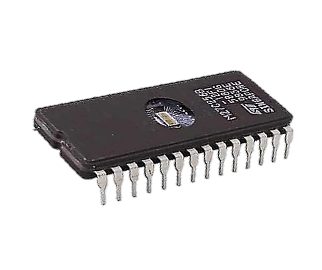
\includegraphics[width=5cm]{Imagens/rom.png}
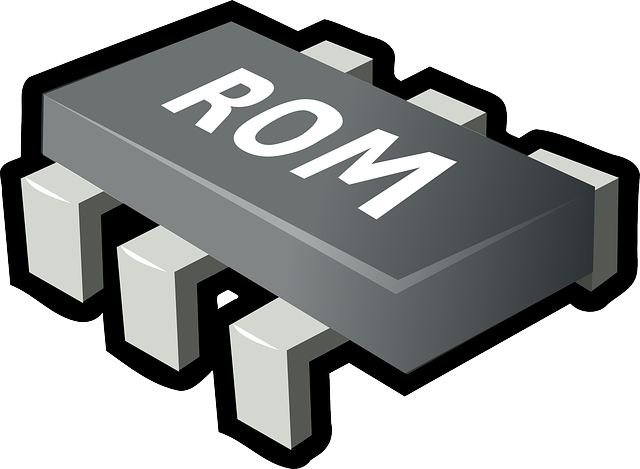
\includegraphics[width=5cm]{Imagens/rom1.png}
\caption{Memória \ac{rom}}
\end{figure}

\newpage

\section{Memória Cache}
\label{sect.cache}

\begin{itemize}
\item Memória principal;
\item Memória volátil (temporária);
\item Dispositivo eletrónico;
\item Dispositivo não removível.
\end{itemize}

É um dispositivo de acesso rápido, interno a um sistema, que serve de intermediário entre um operador de um processo e o dispositivo de armazenamento ao qual esse operador acede, sendo essencial ao bom funcionamento da unidade da qual faz parte.
A vantagem no uso da cache consiste em evitar o acesso ao dispositivo de armazenamento (que pode ser demorado), armazenando os dados em meios de acesso mais rápidos.
Este tipo de memória é de alta velocidade e tem por função armazenar dados e instruções que o processador poderá precisar em breve. Ela possibilita que o processador trabalhe com toda a capacidade.
Cada fabricante utiliza a memória cache de uma forma diferente. Isso também pode variar de acordo com a microarquitetura usada no chip. No entanto, o padrão é que, quando o processador precisa de ir buscar a sua primeira instrução, ele terá de ir até à memória \ac{ram}, visto que a memória cache estará vazia.
Apesar disso, em vez de trazer apenas a solicitação feita pelo processador, a unidade de busca traz um bloco inteiro de instruções que, por sua vez, é armazenado na memória cache. Assim, se o processador continuar a executar o referido programa, as instruções subsequentes estarão já armazenadas na memória cache. Então, a unidade de busca não precisará de ir até à memória \ac{ram} para obtê-las.
Nem sempre a unidade de busca armazena as informações corretas na memória cache. No entanto, a taxa de sucesso é bem alta, cerca de 80\% a 99\% das vezes. Com isso, é possível afirmar que quase todo o acesso à memória RAM é feito através da memória cache.

\begin{figure}[H]
\center
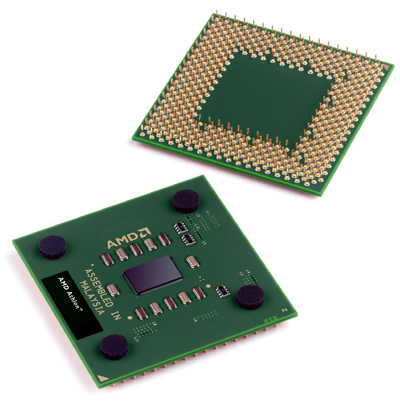
\includegraphics[width=5cm]{Imagens/cache.JPG}
\caption{Memória cache}
\end{figure}

\newpage

\chapter{Evolução}
\label{chap.evolucao}

\paragraph*{}Com a evolução tecnológica os dispositivos de armazenamento estão cada vez menores no tamanho e maiores na capacidade.

\paragraph{}De facto, desde a disquete ao \ac{hd} externo, do \ac{cd} e \ac{dvd} até à pen, o tamanho físico reduziu significativamente mas, mais que isso, a capacidade de armazenamento aumentou em cerca de 2 912 711 vezes! Isto aconteceu devido à evolução da tecnologia, ao aparecimento de ficheiros, programas, dados cada vez mais complexos e detalhados. Claro que este tipo de arquivos também ocupava substancialmete mais espaço e como tal foi necessário o desenvolvimento de dispositivos de armazenamento com cada vez mais memória. Aliada à questão da memória estava a mobilidade. De novo a evolução da tecnologia fez com que os dados deixassem de poder estar parados num dispositivo e em vez disso tivessem que ser movidos, partilhados com outros dispositivos. Claro que toda esta evolução acarreta vários custos, não só a nível monetário, mas também ao nível de preservar esses arquivos ao longo dos anos, pois nem todas as inovações que surgem são compatíveis entre si. 

\begin{figure}[H]
\center
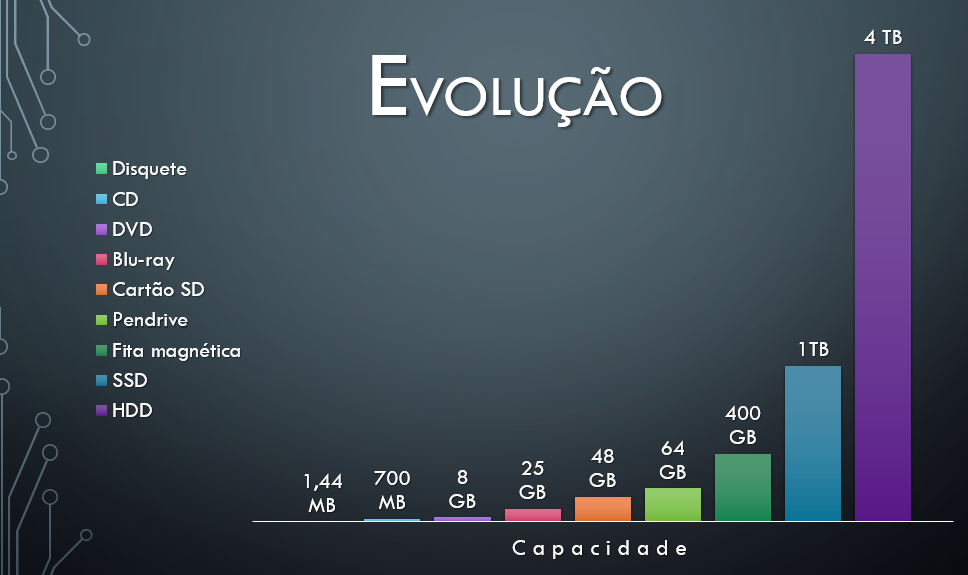
\includegraphics[height=6cm]{Imagens/grafico1.png}
\caption{Gráfico sobre evolução da capacidade dos dispositivos de armazenamento}
\end{figure}

\chapter{Conclusão}
\label{chap.conclusao}
\paragraph*{}Com a realização deste trabalho concluimos que os dispositivos de armazenamento estão em constatnte evolução. O que hoje nós consideramos tecnologia de ponta pode rapidamente ser substituído por algo melhor, mais cómodo, mais rápido e, claro, com mais capacidade de armazenamento. É impossível dizer até onde estes dispositivos podem evoluir pois a sua evolução depende da necessidade de os utilizar. Atualmente os dispositivos de armazenamento que existem chegam para suprir as nossas necessidades mas dentro em breve, com o aparecimento de ficheiros cada vez maiores, vão deixar de ser suficientes. E estes dispositivos vão evoluir, ainda que de maneira incerta, para algo com mais capacidade de armazenamento. Quem sabe, talvez até mais que aquela que precisamos.

\chapter*{Contribuições dos autores}
\paragraph*{}O \ac{js} aplicou as alterações necessárias ao \textit{template} fornecido para o início da escrita em \LaTeX , elaborou o resumo (\textit{abstract}) e realizou a escrita do \autoref{chap.definicao} na totalidade, do \autoref{chap.classificacao} na totalidade e, finalmente, de metade do \autoref{chap.exemplos} (mais detalhadamente: a \autoref{sect.disquete}, a \autoref{sect.cd}, a \autoref{sect.dvd}, a \autoref{sect.bluray}, a \autoref{sect.cartaomemoria} e a \autoref{sect.pen}).

\paragraph*{}O \ac{mn} tratou da redação da segunda metade do \autoref{chap.exemplos} (mais concretamente: a \autoref{sect.hdd}, a \autoref{sect.ssd}, a \autoref{sect.externo}, a \autoref{sect.ram}, a \autoref{sect.rom}, a \autoref{sect.cache}) e da totalidade do \autoref{chap.evolucao}. Além disso, atualizou também o repositório com a versão final do documento.

\paragraph*{}Ambos os membros do grupo contribuiram para a pesquisa dos tópicos a abordar neste documento.
Os dois também trataram da inserção das figuras, utilização de acrónimos e escrita da bibliografia. 
A introdução (\autoref{chap.introducao}) e a conclusão (\autoref{chap.conclusao}) foi redigida pelos dois em simultâneo, através de trocas de ideias para uma melhor escrita. 

\paragraph*{}Em suma, o \ac{js} e o \ac{mn} fizeram 50\% do trabalho cada um, sendo que o \ac{mn} ficou encarregue do envio do PDF final e de todo o restante material deste trabalho de aprofundamento para o eLearning.

\chapter*{Acrónimos}
\begin{acronym}
\acro{labi}[LABI]{Laboratórios de Informática}
\acro{cd}[CD]{Compact Disc}
\acro{dvd}[DVD]{Digital Video Disc}
\acro{sd}[SD]{Secure Digital}
\acro{sdhc}[SDHC]{Secure Digital High Capacity}
\acro{sdxc}[SDXC]{Secure Digital eXtended Capacity}
\acro{usb}[USB]{Universal Serial Bus}
\acro{hdd}[HDD]{Hard Disk Drive}
\acro{hd}[HD]{Hard Disk}
\acro{ssd}[SSD]{Solid State Drive}
\acro{ram}[RAM]{Random Access Memory}
\acro{rom}[ROM]{Read Only Memory}
\acro{bios}[BIOS]{Basic Input/Output System}
\acro{kb}[kB]{Quilobytes}
\acro{mb}[MB]{Megabytes}
\acro{gb}[GB]{Gigabytes}
\acro{tb}[TB]{Terabytes}
\acro{js}[JS]{João Tomás Simões}
\acro{mn}[MN]{Martim Neves}
\end{acronym}

\begin{thebibliography}{9}

\bibitem{1} 
\textbf{Vinicius Buffolo - SlideShare},
\textit{Dispositivos de armazenamento} 
\\\texttt{\url{https://pt.slideshare.net/ViniciusBuffolo/dispositivos-de-armazenamento?qid=502c9ebe-86b4-4b27-9e7e-1c507f3c6f7e}}
 
\bibitem{2} 
\textbf{Vox Tecnologia - SlideShare},
\textit{Introdução à Informática - Módulo 4 - Memórias e Dispositivos de Armazenamento}
\\\texttt{\url{https://pt.slideshare.net/fagnerlima91/introduo-informtica-mdulo-4-memrias-e-dispositivos-de-armazenamento?qid=502c9ebe-86b4-4b27-9e7e-1c507f3c6f7e}}
 
\bibitem{3} 
\textbf{Nuno Pereira - SlideShare},
\textit{A evolução dos dispositivos de armazenamento}
\\\texttt{\url{https://pt.slideshare.net/NunoPereira5/a-evoluo-dos-dispositivos-de-armazenamento-9642312?qid=502c9ebe-86b4-4b27-9e7e-1c507f3c6f7e}}

\bibitem{4} 
\textbf{Felipe Faleiro - SlideShare},
\textit{Dispositivos de armazenamento}
\\\texttt{\url{https://pt.slideshare.net/felipefaleiro/dispositivos-de-armazenamento-53759407?qid=502c9ebe-86b4-4b27-9e7e-1c507f3c6f7e}}

\bibitem{5} 
\textbf{Prefeitura Municipal de Uberaba - SlideShare},
\textit{Multimeios}
\\\texttt{\url{https://pt.slideshare.net/julyanaborges/multimeios?qid=502c9ebe-86b4-4b27-9e7e-1c507f3c6f7e}}

\bibitem{6} 
\textbf{Sotero Pestana - Aplicacões Informáticas B},
\textit{Dispositivos de entrada/saída e de armazenamento}
\\\texttt{\url{https://sites.google.com/site/aplicacoesinformaticasb13/grupo4}}

\bibitem{7} 
\textbf{Wikipédia},
\textit{Dispositivo de armazenamento}
\\\texttt{\url{https://pt.wikipedia.org/wiki/Dispositivo_de_armazenamento}}

\bibitem{8} 
\textbf{José Jardel},
\textit{Disp. Armazenamento - Sistemas de Informação}
\\\texttt{\url{https://jose-jardel.weebly.com/disp-armazenamento.html}}

\bibitem{9} 
\textbf{Enciclopédia Culturama},
\textit{Dispositivo de Armazenamento - Definição, conceito, significado, o que é Dispositivo de Armazenamento}
\\\texttt{\url{https://edukavita.blogspot.pt/2013/01/definicao-de-armazenamento-do.html}}

\bibitem{10} 
\textbf{Mário Armão Ferreira - PCManias},
\textit{SSD vs HDD – Diferenças e vantagens e desvantagens de cada um}
\\\texttt{\url{http://pcmanias.com/ssd-vs-hdd-diferencas-e-vantagens-e-desvantagens-de-cada-um/}}

\bibitem{11} 
\textbf{Daniel Madeira - Dan Scientia},
\textit{O que são dispositivos de armazenamento?}
\\\texttt{\url{http://dan-scientia.blogspot.pt/2010/07/o-que-sao-dispositivos-de-armazenamento.html}} 

\bibitem{12} 
\textbf{Wikipédia},
\textit{Memória (informática)}
\\\texttt{\url{https://pt.wikipedia.org/wiki/Mem\%C3\%B3ria_(inform\%C3\%A1tica)}}

\bibitem{13} 
\textbf{Júlio Monteiro - TechTudo},
\textit{O que é memória RAM e qual é sua função?}
\\\texttt{\url{http://www.techtudo.com.br/artigos/noticia/2012/02/o-que-e-memoria-ram-e-qual-sua-funcao.html}}

\bibitem{14} 
\textbf{Wikipédia},
\textit{Memória somente de leitura}
\\\texttt{\url{https://pt.wikipedia.org/wiki/Mem\%C3\%B3ria_somente_de_leitura}}

\bibitem{15} 
\textbf{Felipe Arruda - TecMundo},
\textit{O que é memória ROM?}
\\\texttt{\url{https://www.tecmundo.com.br/memoria/9346-o-que-e-memoria-rom-.htm}}

\bibitem{16} 
\textbf{NotePlace},
\textit{O que é HD externo e para que serve?}
\\\texttt{\url{http://www.noteplace.com.br/artigo/o-que-e-hd-externo-e-para-que-serve}}

\bibitem{17} 
\textbf{Helito Bijora - TechTudo},
\textit{O que é memória cache? Entenda sua importância para o PC}
\\\texttt{\url{http://www.techtudo.com.br/noticias/noticia/2016/10/o-que-e-memoria-cache-entenda-sua-importancia-para-o-pc.html}}

\end{thebibliography}

\end{document}